\documentclass[../main.tex]{subfiles} % required, if the Chapter be a seperate doc

\begin{document}
\chapter{Einleitung}\label{ch:einleitung}

\section{Physikalischer Hintergrund}\label{sec:physikalischer-hintergrund}

Das \textbf{Federgesetz} – oder, auf mehrere Gegenstände übertragen, das \textbf{Hookesche Gesetz}\footnote{Gemeint ist Robert Hooke, der das Gesetz 1676 erstmals als Anagramm und 1678 aufgelöst publizierte} – beschreibt ein linear-elastisches Verhalten eines Materials, solange es sich innerhalb seiner elastischen Grenze befindet.

Den Begriff \("\)Federgesetz\("\) verwenden wir hier als Oberbegriff für das Hookesche Gesetz in Bezug auf Federsysteme.
Mit dem Hookeschen Gesetz modellieren wir einen linearen Sonderfall des sogenannten Elastizitätsgesetzes.
\begin{tcolorbox}[
        title=Ausholung für das Elastizitätsgesetz,
        colback=gray!10,
        colframe=gray!50,
        boxrule=0.5pt,
        arc=2mm,
        left=2mm,
        right=2mm,
        top=1mm,
        bottom=1mm,
        fonttitle=\bfseries,
    ]
    Das \textbf{Elastizitätsgesetz} beschreibt, wie sich ein elastisches Material unter Belastung verformt und wie dabei Spannung und Dehnung zusammenhängen.
    Im Vergleich zum Hookeschen Gesetz umfasst es jedoch auch nichtlineare oder zeitabhängige Reaktionen des Materials.
\end{tcolorbox}

Hier ist dieser lineare Sonderfall (Das Federgesetz) nochmals in einer Mathematischen Formel ausgedrückt:

\begin{equation}
    F = D \cdot \Delta l
    \label{eq:federgesetz_formel}
\end{equation}

Wobei ${\Delta l}$ die Dehnung ist, die weiderum von der Kraft ${F}$ abhängig ist.
Aus dieser Abhängigkeit bekommen wir nun die Federkonstante ${D}$, die wir durch ${\frac{F}{\Delta l} = D}$ errechnen können.

Die Federkonstante dient jetzt als Proportionalitätsfaktor in der vorher aufgezeigten Formel~\ref{eq:federgesetz_formel} und beschreibt die Steifigkeit der Feder.

\section{Aufgabenstellung}\label{sec:aufgabenstellung}

Die Arbeit stellt eine Zusammenarbeit der Fächer Physik und Mathematik dar.
Ziel ist es, ein physikalisches Experiment zum Federgesetz durchzuführen, die Messdaten systematisch zu erfassen und anschliessend statistisch auszuwerten.
Der Auftrag besteht darin, einen physikalischen Zusammenhang – das Federgesetz – zu untersuchen und die Ergebnisse mit Literaturwerten zu vergleichen.
Zum schluss erfolgt eine Reflexion über unsere Resultate.
Zusätzliche gibt es von den Teammitgliedern selbst noch jeweils eine Reflexion über die Arbeit.

\section{Verwendete experimentelle Methoden}\label{sec:verwendete-experimentelle-methoden}

Experimente zum Federgesetz tragen im Internet viele Namen, jedoch kann man mit einer Feder nicht viele Differenzen
erzeugen wie einfach mit der Ausdehnung, wenn die Feder unter spannung steht.

\begin{figure}[h]
    \centering
    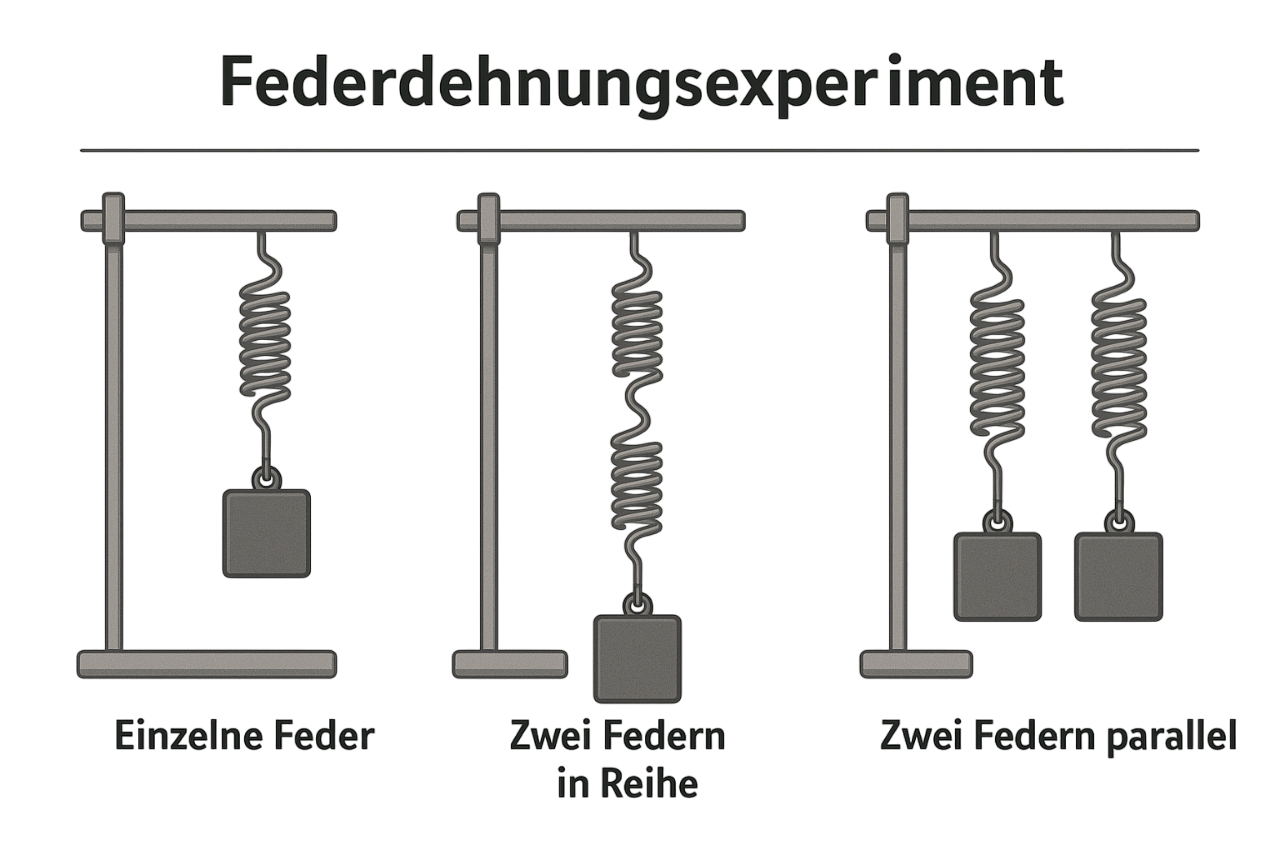
\includegraphics[width=0.7\textwidth]{Federdehungsexperiment}
    \caption{Illustration zum Federdehungsexperiment. Zeigt einzelnen, seriellen und parallelen Teil des Federexperiments. KI generiert für Prompts sehe \ref{sec:generative-ki-nachrichtenverlaufe}}
    \label{fig:mesh1}
\end{figure}

\section{Angewandte statistische Methoden}\label{sec:angewandte-statistische-methoden}

\end{document}
